\documentclass[10pt]{article}
\usepackage[polish]{babel}
\usepackage[utf8]{inputenc}
\usepackage[T1]{fontenc}
\usepackage{amsmath}
\usepackage{amsfonts}
\usepackage{amssymb}
\usepackage[version=4]{mhchem}
\usepackage{stmaryrd}
\usepackage{graphicx}
\usepackage[export]{adjustbox}
\graphicspath{ {./images/} }

\title{XII Konkurs matematyczny St@ś }

\author{}
\date{}


\begin{document}
\maketitle
XIV LO im. Stanisława Staszica\\
4 czerwca 2012 roku

\section*{klasa V}
Na rozwiqzanie poniższych zadań masz 90 minut. Kolejność rozwiazywania tych zadań jest dowolna. Wszystkie zadania sa jednakowo punktowane. Maksymalna liczbę punktów może uzyskać jedynie petne rozwiazanie, z uzasadnieniem \(\boldsymbol{i}\) odpowiedziq.\\
Używanie korektora i korzystanie z kalkulatora jest niedozwolone.

\begin{enumerate}
  \item Butelka z nakrętką kosztuje \(11 \mathrm{zł}\). Butelka jest o \(10 \mathrm{zł}\) droższa od nakrętki. Ile kosztuje nakrętka?
  \item Dany jest trójkąt równoramienny \(A B C(A B=A C)\). Miara kąta \(A\) jest równa \(60^{\circ}\). Na przedłużeniu boku \(B A\) odłożono odcinek \(A D\) tak, że \(A B=A D\).\\
(a) Wyznacz miarę kąta \(B D C\).\\
(b) Wykaż, że trójkąt \(B D C\) jest prostokątny.\\
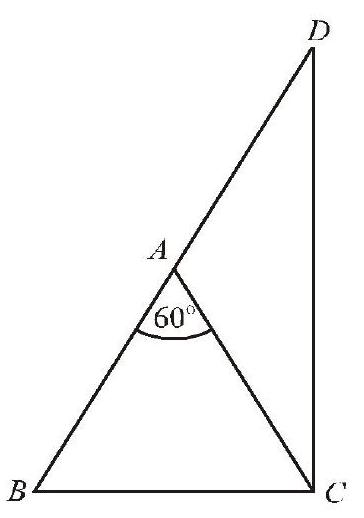
\includegraphics[max width=\textwidth, center]{2024_11_21_6999515b00f050cfcacag-1}
  \item Liczbę naturalną, trzycyfrową zapisano obok tej samej liczby, tak, że otrzymano liczbę sześciocyfrową. Czy ta liczba dzieli się\\
(a) przez 7\\
(b) przez 4?
\end{enumerate}

Odpowiedź uzasadnij.\\
4. Oblicz

\[
2011 \cdot 20122012-2012 \cdot 20112011
\]

\begin{enumerate}
  \setcounter{enumi}{4}
  \item Z jednego wierzchołka sześcianu poprowadzono przekątne dwóch ścian bocznych (tak jak na rysunku). Wyznacz miarę kąta między tymi przekątnymi. Narysuj siatkę tego sześcianu.\\
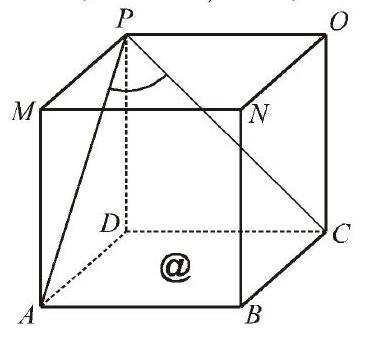
\includegraphics[max width=\textwidth, center]{2024_11_21_6999515b00f050cfcacag-1(1)}
\end{enumerate}

\end{document}